\chapter{Introduction}
\section{Motivation}
\vspace{-0.1cm}
Thanks to recent advancements in Artificial Intelligence (AI), we are now able to leverage Machine Learning and Deep Learning technologies in both academic and commercial applications. Although, relying just on correlations between the different features, can possibly lead to wrong conclusions since correlation does not necessarily imply causation.

Three of the main limitations of nowadays Machine Learning and Deep Learning models are: 
\vspace{-0.2cm}
\begin{itemize}
    \item \textbf{Robustness} = trained models might not be able to generalise to new data and therefore would not be able to provide robust and reliable performances in the real world.
    \item \textbf{Explainability} = complex Deep Learning models can be difficult to analyse in order to clearly demonstrate their decision making process. 
    \item \textbf{Data Dependency} = deep learning models efficiency is highly dependent on the amount and quality of data available. 
\end{itemize}
\vspace{-0.2cm}
Developing models able to identify cause-effect relationships between different variables, might ultimately offer a solution to solve these problems. This idea, has also been supported by researchers such as Judea Pearl and Jonas Peters, which advocated how having models able to reason in uncertainties could not be enough to enable researchers to create machines able to truly express intelligent behaviour \cite{art_perl}.

\section{Going Beyond Correlation}
During the last few years, different approaches have been taken in order to try to overcome correlation limitations. This research focus led then to the development of the "Causality Revolution" and alternative metrics to correlation such as the \textbf{Predictive Power Score (PPS)} \cite{ppc}.

Typical correlation analysis, is able to tell us if there is a linear relationship between different variables by returning a score between -1 (e.g. if one variable increase in values, the other decreases) and 1 (e.g. if one variable increases in value, the other one will follow a similar trend). Although, correlation is not able to identify any non-linear relationship and is not able to handle non-numeric data. In the case of categorical data, this could potentially be converted into numerical data by using for example One Hot Encoding or Word Embedding techniques but would most likely lead to an increase of the dataset dimensionality in order to achieve good results. Finally, correlation might not be able to understand if relationships between the different columns are symmetric or asymmetric.

In Figure \ref{corr_t}, is available a summary of some examples of correlation trends and limitations.

\vspace{-0.1cm}
\begin{figure}[ht!]%
    \centering
    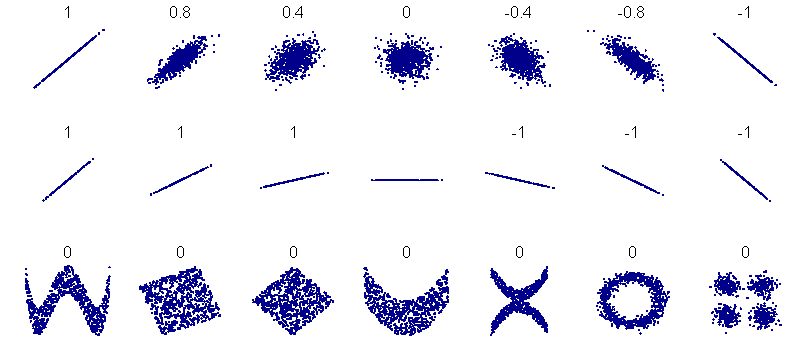
\includegraphics[width=0.85\linewidth]{latex/images/corr.pdf}
    % 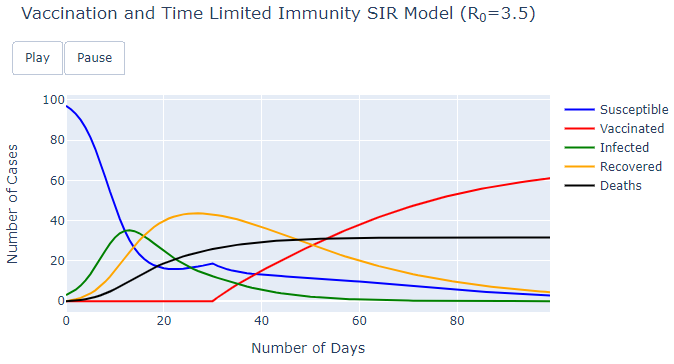
\includegraphics[width=13cm]{latex/images/vacc.PNG}%
    \vspace{-0.2cm}
    \caption{Correlation Trends (Image reproduced from \cite{corr_trends})}
    \label{corr_t}
\end{figure}
\vspace{-0.5cm}

The predictive power score, has been ideated in order to try to overcome the presented correlation limitations. One possible way to calculate the PPS is to train a Cross-Validated Decision Tree model on one feature and consider the other feature we want to consider as our label. We can then evaluate the model using an appropriate evaluation metric and then normalise the score by comparing it with the score obtained by a naive predictor. A possible set-up for a PPS calculation is shown in Table \ref{setup}.

{
\begin{table}[h!]
\centering
\begin{tabular}{l|l|c|c|c}
\multicolumn{2}{c}{}&\multicolumn{2}{c}{}&\\
\cline{3-4}
\multicolumn{2}{c|}{}&Numeric Data &Categorical Data &\multicolumn{1}{c}{}\\
\cline{2-4}
\multirow{}{}{}& ML Model & Decision Tree Regressor & Decision Tree Classifier & \\
\cline{2-4}
& Evaluation Metric & Mean Absolute Error & Weighted F1 Score & \\
\cline{2-4}
& Naive Predictor & Predict median value & Predict most common class & \\
\cline{2-4}
% \multicolumn{1}{c}{} & \multicolumn{1}{c}{} & \multicolumn{1}{c}{} & \multicolumn{1}{c}{} & \multicolumn{1}{c}{}\\
\end{tabular}
% \vspace{-0.7cm}
\caption{Predictive Power Score Set-up}
\label{setup}
\end{table}
}

Where the Mean Absolute Error (MAE) and F1 score can be defined as:

\useshortskip
\begin{align}
\ F1 = 2 \times \dfrac{precision \times recall}{precision + recall}
\ MAE = \dfrac{1}{n}\sum_{i=1}^{n}\abs{x_{i} - x}
\end{align}
\useshortskip

The result from the evaluation metric, can then be normalised by comparing it with the results from the naive predictor. In the case of the F1 Score, 1 is going to be considered our upper limit and the naive predictor score as our lower limit.

\useshortskip
\begin{align}
\ PPS = \dfrac{Decision\:Tree\:(F1) - Naive\:Predictor\:(F1)}{1 - Naive\:Predictor\:(F1)}
\end{align}
\useshortskip

A similar formula could then be calculated for the MAE case, but zero should be considered as our lower limit (in this case, lower scores are considered as better).

\useshortskip
\begin{align}
\ PPS = 1 - \dfrac{Decision\:Tree\:(MAE)}{Naive\:Predictor\:(MAE)}
\end{align}
\useshortskip

Following this procedure, we would then have a PPS score between 0 (no relationship) and 1 (perfect relationship) able to capture either linear/non-linear relationships and to work with either numerical or categorical data. 

As a simple demonstration of the PPS score, is shown in Figure \ref{pps_ex} a noisy cosine function. In this example, the X axis has been created by creating a uniform range between 0 and 1000, while the Y axis has been created by passing the respective X value in a cosine function and adding some small noise on the result. In this way, is designed a clear non-linear dependence between X and Y. 

Calculating the correlation between the two features, would then lead to a result equal to zero (from either points of view). Using instead the PPS, would the lead as expected to a score of 0.737 of X respect to Y and of 0 for Y respect to X. 

% \vspace{-0.1cm}
\begin{figure}[ht!]%
    \centering
    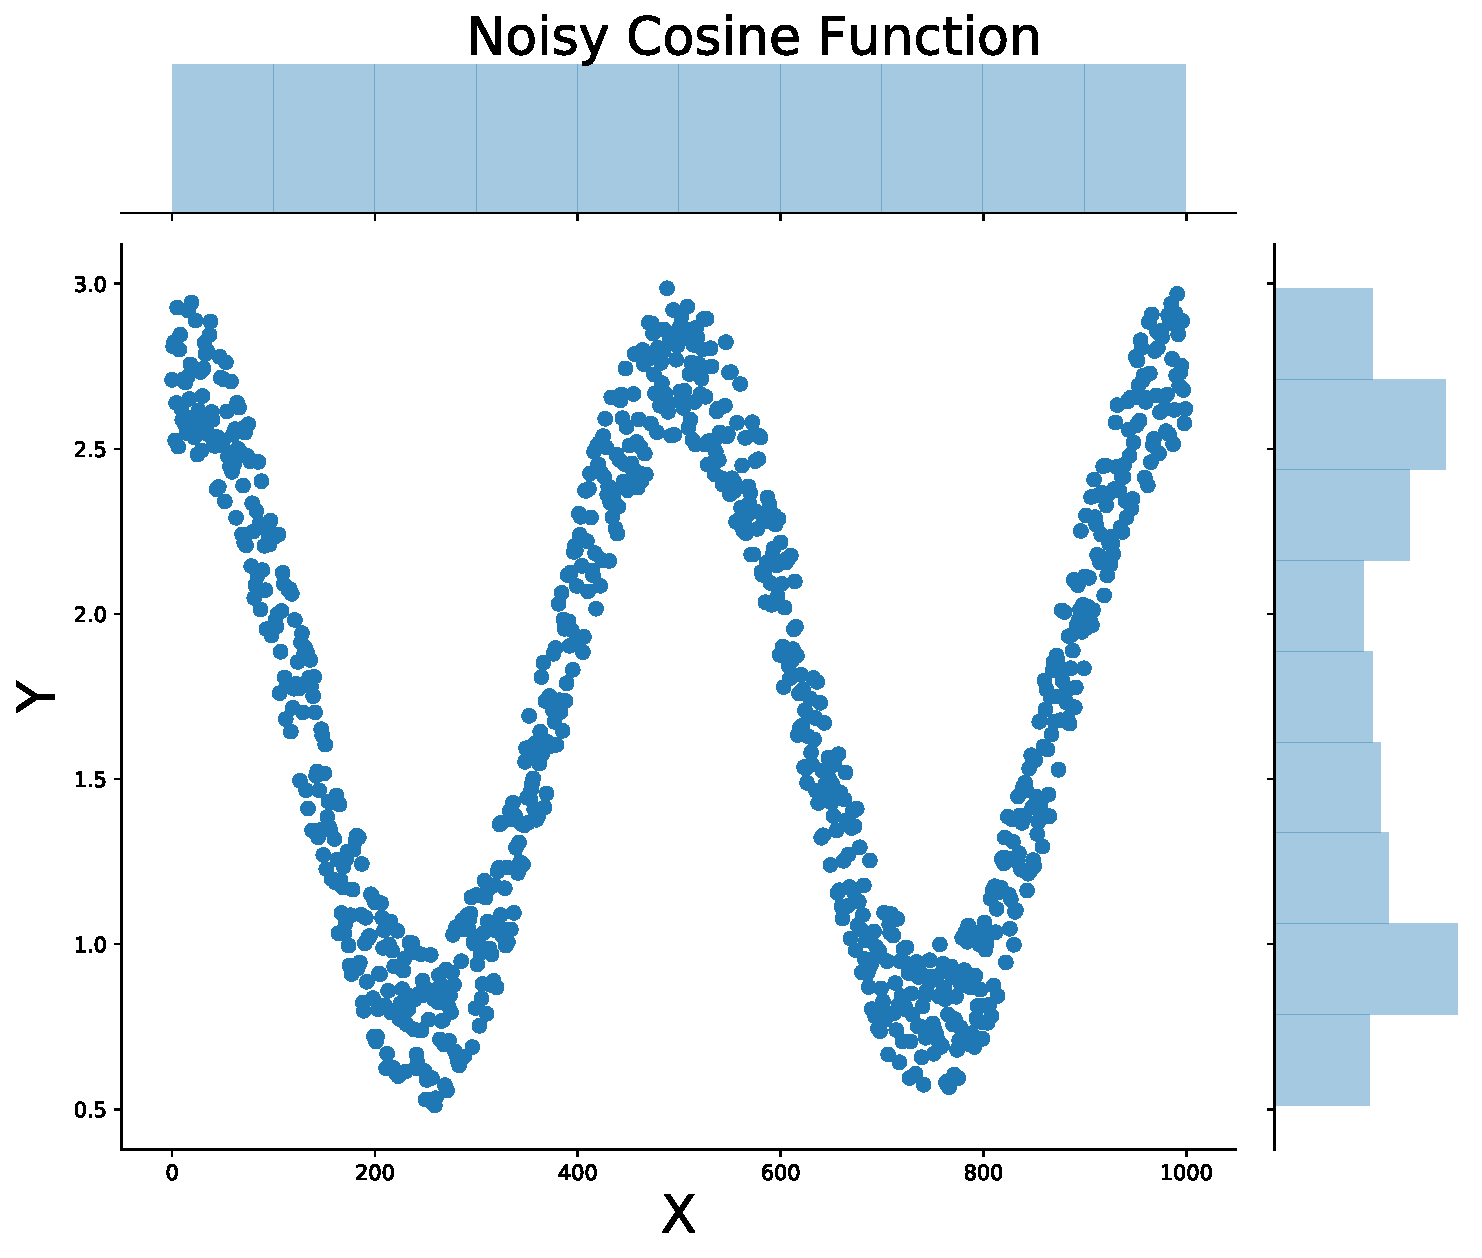
\includegraphics[width=0.45\linewidth]{latex/images/pps_ex.pdf}
    % 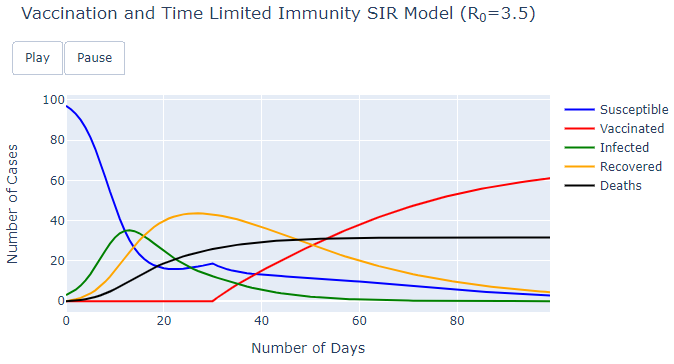
\includegraphics[width=13cm]{latex/images/vacc.PNG}%
    \vspace{-0.2cm}
    \caption{PPS Score Example}
    \label{pps_ex}
\end{figure}
% \vspace{-0.1cm}

The Predictive Power Score, is just one of the different approaches which can be taken in order to go beyond correlation traditional limitations, other examples are: Causality, relative entropy and Granger techniques.

\section{Causality vs Explainability}
One of the major trade-offs in nowadays Machine Learning is model performance against complexity. In fact, complex Deep Learning architectures are usually able to perform better in a wide variety of tasks compared to traditional linear classifiers and regression techniques. This trade-off has been analysed in-depth in the 2016 publication "Why should I trust you?" by Ribiero et. al. \cite{otto} and led a new trend in AI to focus on interpretability.

Complex and more accurate models are nowadays referred to as \textbf{Black-boxes}. These type of models working progresses are more difficult to comprehend and they are not able to estimate the importance of each feature and how they are related to each other. Some examples of Black Boxes models are neural networks and ensemble models.

On the other hand, simpler and less accurate models such as decision trees and linear regression, are instead regarded as \textbf{White-boxes} and can be much more interpretable. Two of the main measures which can be used in order to estimate the explainability of a model, are the linearity and monotonicity of a model response function \cite{nove}.

One of the key differences between Explainable AI and Causal AI, is that the former aims just to understand how a model might come to a prediction by weighting the provided features while the latter is designed undercover the process governing the system we are analysing to create insights. In this way, Causal AI can be used in order to answer common retrospective and system design type of questions, providing vital business value to organizations (e.g. EU’s General Data Protection Regulation, right to explanation clause) \cite{causalens}. 

\section{Objectives}
\vspace{-0.1cm}
As part of this research study, will be outlined the main principles of Causal Reasoning and different application approaches (e.g. Bayesian Belief Networks, Time Series Analysis) and an Epidemic Modelling case study concerning COVID-19 (Coronavirus). The Novel Coronavirus, is new type of RNA virus which can be able to infect humans potentially causing respiratory infections. The 2020 Novel Coronavirus outbreak started in the late 2019 in Wuhan, China and, as of July 2020, it is believed the virus is mainly able to spread by air through sneezing and coughing. 